% !TeX program = lualatex
\documentclass[11pt,a4paper]{article}
\usepackage{szzmaterial}
\usetikzlibrary{calc}
\setlist[enumerate]{nosep,leftmargin=2.1em}
\setlist[itemize]{nosep,leftmargin=1.8em}

\szztitul{Algebra a lineární algebra}{M2}{NMAI057 (Lineární algebra 1), NMAI058 (Lineární algebra 2)}

\newcommand{\playlist}{https://www.youtube.com/playlist?list=PLZHQObOWTQDPD3MizzM2xVFitgF8hE_ab}
\newcommand{\rank}{\operatorname{rank}}
\newcommand{\Ker}{\operatorname{Ker}}
\newcommand{\sgn}{\operatorname{sgn}}
\newcommand{\spn}{\operatorname{span}}
\newcommand{\tr}{\operatorname{trace}}

\begin{document}
\maketitle
\tableofcontents
\bigskip

\section*{Úvod}
\addcontentsline{toc}{section}{Úvod}

Tento materiál pokrývá okruh \textbf{M2 -- Algebra a lineární algebra} (předměty NMAI057 a NMAI058, Lineární algebra 1 a~2). Výklad je postaven primárně na učebnici doc.~Milana Hladíka \emph{Lineární algebra (nejen) pro informatiky}, podle níž se kurz vyučuje; značení a hloubka odpovídají kurzu pro informatiky (tedy ne rigor matematických oborů). Důraz a rozsah jsme porovnali s~\emph{Podrobným minimálním sylabem přednášek Lineární algebra I a~II pro informatiky} (J.~Matoušek).

Věty uvádíme \emph{se zněním}, doplněné intuicí a krátkými odvozeními tam, kde pomáhají pochopení; rozsáhlé formální důkazy vynecháváme. Do výkladu jsou zařazeny řešené reálné otázky SZZ z let 2022--2026; všechny otázky k okruhu jsou pohromadě v samostatném dokumentu \emph{Příklady otázek}. Použité zdroje jsou uvedeny na konci.

\medskip
\noindent\textbf{Značení.} Tělesa značíme $T$, nejčastěji $\mathbb{R}$ (reálná čísla), $\mathbb{C}$ (komplexní), $\mathbb{Z}_p$ (zbytkové třídy modulo prvočíslo). Matice značíme velkými písmeny, $A\in T^{m\times n}$, prvek na pozici $(i,j)$ je $a_{ij}$ nebo $A_{ij}$; $A_{i*}$ je $i$-tý řádek, $A_{*j}$ je $j$-tý sloupec. Vektory jsou malá písmena, standardně sloupcové, $x\in T^n$; $e_i$ je $i$-tý jednotkový vektor, $I_n$ jednotková matice řádu $n$, $o$ nulový vektor. Transpozice je $A^T$, inverze $A^{-1}$, hodnost $\rank(A)$.

\video{\playlist}{3Blue1Brown -- Essence of Linear Algebra (celá série dává vizuální intuici k vektorům, lineárním zobrazením, determinantu a vlastním vektorům; odkazujeme na konkrétní díly u jednotlivých témat).}

% ============================================================
\section{Algebraické struktury (grupy, tělesa, konečná tělesa)}

Lineární algebra pracuje s vektory, které umíme sčítat a násobit skalárem. \uv{Skaláry} berou z nějakého tělesa a samotné sčítání tvoří strukturu zvanou grupa. Než tedy zavedeme vektorové prostory, popíšeme tyto dvě algebraické struktury. Obě se definují \emph{axiomaticky}: vyjmenujeme vlastnosti, které mají operace splňovat, a strukturou pak je cokoli, co je splňuje. Výhoda je, že vše, co z axiomů odvodíme, platí naráz pro všechny konkrétní případy.

\subsection{Grupy a permutace}

\begin{definice}[Grupa]
\emph{Grupa} je dvojice $(G,\circ)$, kde $G$ je množina a $\circ:G\times G\to G$ binární operace splňující
\begin{enumerate}[label=(\arabic*)]
  \item $\forall a,b,c\in G:\ a\circ(b\circ c)=(a\circ b)\circ c$ \quad (asociativita),
  \item $\exists e\in G\ \forall a\in G:\ e\circ a=a\circ e=a$ \quad (existence neutrálního prvku),
  \item $\forall a\in G\ \exists b\in G:\ a\circ b=b\circ a=e$ \quad (existence inverzního prvku).
\end{enumerate}
Grupa je \emph{Abelova} (komutativní), splňuje-li navíc $a\circ b=b\circ a$ pro všechna $a,b\in G$.
\end{definice}

\begin{intuice}
V definici je skrytá podmínka \emph{uzavřenosti}: výsledek $a\circ b$ nesmí \uv{vypadnout} z~$G$. Píšeme-li operaci jako sčítání, neutrální prvek značíme $0$ a inverzní $-a$; píšeme-li ji jako násobení, neutrální prvek je $1$ a inverzní $a^{-1}$.
\end{intuice}

\begin{priklad}[Grupy a negrupy]
$(\mathbb{Z},+)$, $(\mathbb{Q},+)$, $(\mathbb{R},+)$, $(\mathbb{R}^{m\times n},+)$ a $(\mathbb{Z}_n,+)$ (sčítání modulo~$n$) jsou Abelovy grupy. $(\mathbb{R}\setminus\{0\},\cdot)$ je Abelova grupa (nulu musíme vynechat, nemá inverzi). Neabelovské příklady: regulární matice řádu $n$ s násobením, nebo permutace s~skládáním. Naopak $(\mathbb{N},+)$ grupa není (chybí inverzní prvky).
\end{priklad}

\begin{definice}[Podgrupa]
$(H,\circ)$ je \emph{podgrupa} grupy $(G,\circ)$, pokud $H\subseteq G$ a $H$ se stejnou operací sama tvoří grupu; tj. $H$ obsahuje $e$, je uzavřená na $\circ$ a na inverze. Značíme $(H,\circ)\le(G,\circ)$.
\end{definice}

\begin{veta}[Základní vlastnosti grupy]
V každé grupě $(G,\circ)$ platí:
\begin{itemize}
  \item neutrální prvek je jediný a~ke každému prvku existuje jediný inverzní;
  \item \emph{krácení}: $a\circ c=b\circ c\Rightarrow a=b$;
  \item rovnice $a\circ x=b$ má právě jedno řešení;
  \item $(a^{-1})^{-1}=a$ a $(a\circ b)^{-1}=b^{-1}\circ a^{-1}$.
\end{itemize}
\end{veta}

Důležitým příkladem neabelovské grupy jsou permutace.

\begin{definice}[Permutace a její znaménko]
\emph{Permutace} na množině $\{1,\dots,n\}$ je bijekce $p:\{1,\dots,n\}\to\{1,\dots,n\}$; množinu všech takových permutací značíme $S_n$. Permutaci lze rozložit na disjunktní \emph{cykly}. \emph{Transpozice} $(i,j)$ je permutace s jediným netriviálním cyklem délky~2. Skládá-li se $p$ z $k$ cyklů (včetně jednoprvkových), je její \emph{znaménko} $\sgn(p)=(-1)^{n-k}$.
\end{definice}

\begin{poznamka}
Znaménko je vždy $\pm1$; permutace se znaménkem $+1$ jsou \emph{sudé}, se znaménkem $-1$ \emph{liché}. Každou permutaci lze rozložit na složení transpozic a platí $\sgn(p)=(-1)^r$, kde $r$ je počet transpozic v rozkladu (jejich \emph{parita} je jednoznačná, počet ne). Klíčová vlastnost pro determinanty: $\sgn(p\circ q)=\sgn(p)\,\sgn(q)$. Množina $(S_n,\circ)$ tvoří tzv. \emph{symetrickou grupu}, pro $n\ge3$ nekomutativní.
\end{poznamka}

\subsection{Tělesa a konečná tělesa}

Zatímco grupa má jednu operaci, těleso má dvě (sčítání a~násobení) jako například $\mathbb{R}$. Díky tělesu můžeme s maticemi a~soustavami pracovat i nad jinými obory než reálnými čísly.

\begin{definice}[Těleso]
\emph{Těleso} je množina $T$ se dvěma komutativními binárními operacemi $+$ a $\cdot$ takovými, že
\begin{enumerate}[label=(\arabic*)]
  \item $(T,+)$ je Abelova grupa (neutrální prvek $0$, inverzní $-a$),
  \item $(T\setminus\{0\},\cdot)$ je Abelova grupa (neutrální prvek $1$, inverzní $a^{-1}$),
  \item $\forall a,b,c\in T:\ a\cdot(b+c)=a\cdot b+a\cdot c$ \quad (distributivita).
\end{enumerate}
\end{definice}

\begin{intuice}
Těleso je obor, ve kterém lze \uv{počítat jako s čísly}: sčítat, odčítat, násobit a dělit nenulovými prvky. Každé těleso má aspoň dva prvky ($0\neq1$). $\mathbb{Q},\mathbb{R},\mathbb{C}$ jsou tělesa; $\mathbb{Z}$ těleso není (chybí inverze k násobení, např. $2^{-1}\notin\mathbb{Z}$). Z axiomů plyne $0a=0$ a \uv{nulovost součinu}: $ab=0\Rightarrow a=0$ nebo $b=0$.
\end{intuice}

\begin{priklad}[Konečné těleso $\mathbb{Z}_n$]
Na množině $\mathbb{Z}_n=\{0,1,\dots,n-1\}$ definujeme $+$ a $\cdot$ modulo $n$. $\mathbb{Z}_2,\mathbb{Z}_3$ jsou tělesa, ale $\mathbb{Z}_4$ není (prvek $2$ nemá inverzi).
\end{priklad}

\begin{veta}[Kdy je $\mathbb{Z}_n$ těleso]
$\mathbb{Z}_n$ je těleso právě tehdy, když $n$ je prvočíslo.
\end{veta}

\begin{intuice}
Je-li $n=pq$ složené ($1<p,q<n$), pak $p\cdot q=0$ v~$\mathbb{Z}_n$, ač $p,q\neq0$ -- to porušuje nulovost součinu, kterou každé těleso splňuje. Pro prvočíslo $n$ naopak inverze vždy existuje: násobky $\{0a,1a,\dots,(n-1)a\}$ nenulového $a$ proběhnou všechny zbytky, takže mezi nimi je i~$1=ba$, a tedy $b=a^{-1}$.
\end{intuice}

\begin{poznamka}[Velikost konečných těles a charakteristika]
Konečná tělesa existují právě o velikostech $p^n$, kde $p$ je prvočíslo a $n\ge1$; značí se $GF(p^n)$ (Galoisovo těleso) a každé dvě téže velikosti jsou isomorfní. \emph{Charakteristika} tělesa je nejmenší $n$ s $\underbrace{1+\dots+1}_{n}=0$ (a~$0$, pokud takové $n$ neexistuje); je buď nula (jako u $\mathbb{Q},\mathbb{R},\mathbb{C}$), nebo prvočíslo (u $\mathbb{Z}_p$ je rovna~$p$). Pro informatiku je klíčové $\mathbb{Z}_2=\{0,1\}$: sčítání odpovídá XOR, násobení AND.
\end{poznamka}

\begin{priklad}[Inverze v $\mathbb{Z}_5$ a malá Fermatova věta]
V $\mathbb{Z}_5$ jsou inverze pro násobení: $1^{-1}=1$, $2^{-1}=3$ (neboť $2\cdot3=6\equiv1$), $3^{-1}=2$, $4^{-1}=4$. \emph{Malá Fermatova věta}: pro prvočíslo $p$ a $0\neq a\in\mathbb{Z}_p$ platí $a^{p-1}=1$. Příklad: $2^{111}$ v $\mathbb{Z}_{11}$. Protože $2^{10}=1$, je $2^{110}=1$, takže $2^{111}=2^{110}\cdot2=2$.
\end{priklad}

\begin{priklad}[Znaménko permutace a kdy je $\mathbb{Z}_n$ těleso]
\begin{itemize}
  \item[(a)] Permutace $p\in S_5$ daná rozkladem na cykly $p=(1\,3\,2)(4\,5)$ má dva cykly (délek $3$ a~$2$), tedy $\sgn(p)=(-1)^{5-2}=-1$ -- je lichá. Totéž z~rozkladu na transpozice: $(1\,3\,2)=(1\,3)(3\,2)$ a~$(4\,5)$ dají dohromady $3$ transpozice, $\sgn(p)=(-1)^3=-1$.
  \item[(b)] $\mathbb{Z}_5$ je těleso ($5$ je prvočíslo). $\mathbb{Z}_6$ těleso \emph{není}: $6=2\cdot3$ je složené a~v~$\mathbb{Z}_6$ platí $2\cdot3=0$, ačkoli $2,3\neq0$ -- to porušuje nulovost součinu (a~prvek $2$ nemá inverzi).
\end{itemize}
\end{priklad}

% ============================================================
\section{Soustavy lineárních rovnic (Gaussova eliminace)}

Soustavy lineárních rovnic jsou základní úlohou; zapisujeme je maticově a řešíme elementárními úpravami.

\begin{definice}[Soustava a její matice]
\emph{Soustava $m$ lineárních rovnic o $n$ neznámých} nad tělesem $T$ je
\[
  a_{11}x_1+\dots+a_{1n}x_n=b_1,\quad\dots,\quad a_{m1}x_1+\dots+a_{mn}x_n=b_m,
\]
maticově $Ax=b$, kde $A\in T^{m\times n}$ je \emph{matice soustavy}, $b\in T^m$ vektor pravých stran. \emph{Rozšířená matice soustavy} je $(A\mid b)$. Řešením je každý vektor $x\in T^n$ vyhovující všem rovnicím.
\end{definice}

\begin{definice}[Elementární řádkové úpravy (ERÚ)]
ERÚ matice jsou:
\begin{enumerate}[label=(\arabic*)]
  \item vynásobení řádku nenulovým skalárem $\alpha$;
  \item přičtení $\alpha$-násobku jednoho řádku k~jinému;
  \item výměna dvou řádků.
\end{enumerate}
\end{definice}

\begin{veta}[ERÚ zachovávají množinu řešení]
Provedeme-li na rozšířené matici $(A\mid b)$ elementární řádkovou úpravu, množina řešení soustavy se nezmění.
\end{veta}

\begin{intuice}
Každá ERÚ má svou inverzní úpravu, takže žádné řešení nepřibude ani neubude. Řádky odpovídají rovnicím; sčítání a škálování rovnic je legální, protože nemění jejich řešení.
\end{intuice}

\begin{definice}[Odstupňovaný tvar a hodnost]
Matice je v \emph{řádkově odstupňovaném tvaru} (REF), pokud nenulové řádky předcházejí nulovým a pozice prvních nenulových prvků (\emph{pivotů}) v~řádcích ostře rostou shora dolů. \emph{Hodnost} $\rank(A)$ je počet nenulových řádků (pivotů) po převodu do REF. Sloupce s pivotem jsou \emph{bázické}, ostatní \emph{nebázické}.
\end{definice}

\begin{poznamka}
REF tvar není jednoznačný, ale pozice pivotů ano, takže hodnost je dobře definovaná. Každou matici lze do REF převést Gaussovou eliminací (dopřednou eliminací nul pod pivoty).
\end{poznamka}

\begin{veta}[Gaussova eliminace -- řešitelnost (Frobeniova věta)]
Převedeme $(A\mid b)$ na REF tvar $(A'\mid b')$. Pak:
\begin{itemize}
  \item soustava \emph{nemá řešení} právě tehdy, když $\rank(A)<\rank(A\mid b)$ (pivot v posledním sloupci);
  \item má \emph{právě jedno řešení}, je-li $\rank(A)=\rank(A\mid b)=n$;
  \item má \emph{více než jedno řešení}, je-li $\rank(A)=\rank(A\mid b)=r<n$ (nad nekonečným tělesem jako $\mathbb{R}$ nekonečně mnoho, nad $\mathbb{Z}_p$ právě $p^{\,n-r}$); množinu řešení popíšeme parametricky, kde $n-r$ nebázických (volných) proměnných tvoří parametry a bázické dopočítáme \emph{zpětnou substitucí}. Číslo $n-r$ je dimenze množiny řešení.
\end{itemize}
\end{veta}

\begin{poznamka}[Gaussova--Jordanova eliminace]
\emph{Redukovaný} odstupňovaný tvar (RREF) má navíc na pivotech jedničky a nad pivoty nuly. Gaussova--Jordanova eliminace převádí matici do RREF a řešení z~ní lze odečíst přímo, bez zpětné substituce.
\end{poznamka}

\begin{priklad}[Soustava s nekonečně mnoha řešeními]
\textbf{Zadání.} Vyřešte soustavu s~rozšířenou maticí
\[ \begin{pmatrix} 2&2&-1&5&1\\ 4&5&0&9&3\\ 0&1&2&2&4\\ 2&4&3&7&7 \end{pmatrix}. \]
\textbf{Řešení.} Převodem na odstupňovaný (REF) tvar dostaneme
\[ \begin{pmatrix} 2&2&-1&5&1\\ 0&1&2&-1&1\\ 0&0&0&3&3\\ 0&0&0&0&0 \end{pmatrix}. \]
Hodnost matice i rozšířené matice je $3<4$, soustava má tedy $4-3=1$-parametrickou množinu řešení. Pivoty jsou ve sloupcích $1,2,4$; volná je $x_3$. Zpětnou substitucí $x_4=1$, $x_2=2-2x_3$, $x_1=-4+\tfrac52 x_3$, takže
\[
  (x_1,x_2,x_3,x_4)=(-4,2,0,1)+x_3\bigl(\tfrac52,-2,1,0\bigr),\qquad x_3\in\mathbb{R}.
\]
Význam zápisu (partikulární řešení $+$ obecné řešení homogenní soustavy) vyplyne ze sekce o~vektorových prostorech.
\end{priklad}

% ============================================================
\section{Matice (operace, hodnost, inverzní matice)}

\subsection{Operace a typy matic}

\begin{definice}[Operace s maticemi]
Pro $A,B$ téhož typu a skalár $\alpha$: $(A+B)_{ij}=a_{ij}+b_{ij}$ a $(\alpha A)_{ij}=\alpha a_{ij}$. \emph{Součin} $AB$ matic $A\in T^{m\times p}$, $B\in T^{p\times n}$ je matice typu $m\times n$ s prvky $(AB)_{ij}=\sum_{k=1}^{p}a_{ik}b_{kj}$ (skalární součin $i$-tého řádku $A$ a $j$-tého sloupce $B$). \emph{Transpozice} $A^T$ má $(A^T)_{ij}=a_{ji}$.
\end{definice}

\begin{poznamka}[Vlastnosti]
Sčítání je komutativní a asociativní. Součin je asociativní a distributivní, $I_mA=AI_n=A$, ale \textbf{není komutativní} (obecně $AB\neq BA$). Dále $(AB)^T=B^TA^T$ a $(A+B)^T=A^T+B^T$. Matice $A$ je \emph{symetrická}, je-li $A=A^T$; pro libovolnou $B$ je $B^TB$ symetrická. \emph{Stopa} čtvercové matice je součet jejích diagonálních prvků, $\tr(A)=\sum_i a_{ii}$; platí $\tr(A)=\tr(A^T)$ a~$\tr(AB)=\tr(BA)$ (a~$\tr(A)=\sum_i\lambda_i$, viz sekci o~vlastních číslech).
\end{poznamka}

\begin{intuice}
Násobení matic odpovídá \emph{skládání zobrazení}: díváme-li se na $A$ jako na zobrazení $x\mapsto Ax$, pak $B(Ax)=(BA)x$. Proto je součin asociativní (skládání zobrazení je vždy asociativní) a nekomutativní (na pořadí transformací záleží). To je i historický důvod, proč se součin definuje právě takto.
\end{intuice}

\begin{poznamka}[Speciální matice]
\emph{Diagonální} matice má nuly mimo diagonálu, $\operatorname{diag}(v_1,\dots,v_n)$. \emph{Horní trojúhelníková} má nuly pod diagonálou (každá REF matice je horní trojúhelníková). Matice \emph{hodnosti~1} jsou právě matice tvaru $xy^T$ pro nenulové $x,y$ (každý řádek je násobkem $y^T$).
\end{poznamka}

\subsection{Regulární a inverzní matice}

\begin{definice}[Regulární matice]
Čtvercová $A\in T^{n\times n}$ je \emph{regulární}, má-li homogenní soustava $Ax=o$ jediné řešení $x=o$; jinak je \emph{singulární}.
\end{definice}

\begin{veta}[Charakterizace regularity]
Pro $A\in T^{n\times n}$ jsou ekvivalentní:
\begin{enumerate}[label=(\arabic*)]
  \item $A$ je regulární;
  \item $\mathrm{RREF}(A)=I_n$;
  \item $\rank(A)=n$;
  \item pro každé $b$ má soustava $Ax=b$ právě jedno řešení.
\end{enumerate}
\end{veta}

\begin{definice}[Inverzní matice]
$A^{-1}$ je \emph{inverzní} k $A\in T^{n\times n}$, pokud $AA^{-1}=A^{-1}A=I_n$.
\end{definice}

\begin{veta}[Existence a výpočet inverze]
Matice $A$ má inverzi právě tehdy, když je regulární, a pak je inverze jediná. Spočítáme ji převodem $(A\mid I_n)$ Gaussovou--Jordanovou eliminací: je-li $\mathrm{RREF}(A\mid I_n)=(I_n\mid B)$, pak $B=A^{-1}$ (netvoří-li levá část $I_n$, je $A$ singulární). Platí $(AB)^{-1}=B^{-1}A^{-1}$ a $(A^T)^{-1}=(A^{-1})^T$.
\end{veta}

\begin{intuice}
$j$-tý sloupec $A^{-1}$ je řešením soustavy $Ax=e_j$. Všechny tyto soustavy mají stejnou matici $A$, proto je řešíme naráz s pravou stranou $I_n$. K řešení soustavy $Ax=b$ pak stačí $x=A^{-1}b$ (v praxi se ale řeší rovnou Gaussovou eliminací, je to levnější).
\end{intuice}

\begin{priklad}[Výpočet inverze]
\textbf{Zadání.} Najděte inverzi matice $A=\begin{psmallmatrix}1&1&3\\0&2&-1\\3&5&7\end{psmallmatrix}$.\par
\textbf{Řešení.} Úpravou $(A\mid I_3)$ Gaussovou--Jordanovou eliminací na tvar $(I_3\mid A^{-1})$:
\[
  A^{-1}=\begin{pmatrix}-9.5&-4&3.5\\ 1.5&1&-0.5\\ 3&1&-1\end{pmatrix}.
\]
Ověření: $AA^{-1}=I_3$.
\end{priklad}

% ============================================================
\section{Vektorové prostory (báze, dimenze, podprostory)}

\subsection{Vektorový prostor, podprostor, lineární obal}

\begin{definice}[Vektorový prostor]
\emph{Vektorový prostor nad tělesem $T$} je množina $V$ s~operacemi sčítání $+:V\times V\to V$ a~násobení skalárem $\cdot:T\times V\to V$ takovými, že $(V,+)$ je Abelova grupa (nulový vektor~$o$) a~pro všechna $\alpha,\beta\in T$ a $u,v\in V$ platí:
\begin{enumerate}[label=(\arabic*)]
  \item $\alpha(\beta v)=(\alpha\beta)v$ \quad(asociativita násobení skalárem),
  \item $1v=v$ \quad(jednotkový skalár),
  \item $(\alpha+\beta)v=\alpha v+\beta v$ \quad(distributivita vůči sčítání skalárů),
  \item $\alpha(u+v)=\alpha u+\alpha v$ \quad(distributivita vůči sčítání vektorů).
\end{enumerate}
\end{definice}

\begin{priklad}
Aritmetický prostor $T^n$, prostor matic $T^{m\times n}$, prostor polynomů $\mathcal P^n$ stupně nejvýše~$n$ (dimenze $n+1$), prostor všech polynomů $\mathcal P$ či spojitých funkcí $\mathcal C$ (nekonečné dimenze).
\end{priklad}

\video{https://www.youtube.com/watch?v=TgKwz5Ikpc8}{3Blue1Brown, \emph{Essence of Linear Algebra} kap.~16 -- \emph{Abstract vector spaces} (vektorový prostor abstraktně přes axiomy: polynomy, funkce i~matice jako \uv{vektory}).}

\begin{definice}[Podprostor]
$U\subseteq V$ je \emph{podprostor}, tvoří-li sám vektorový prostor se stejnými operacemi. Ekvivalentně: $o\in U$, a $U$ je uzavřená na součty a na násobky skalárem.
\end{definice}

\begin{definice}[Lineární kombinace, obal, generátory]
\emph{Lineární kombinace} vektorů $v_1,\dots,v_n$ je výraz $\sum_{i=1}^n\alpha_iv_i$ s~$\alpha_i\in T$. \emph{Lineární obal} $\spn(W)$ je nejmenší podprostor obsahující $W$; pro konečné $W=\{v_1,\dots,v_n\}$ je $\spn(W)=\{\sum\alpha_iv_i\}$ (všechny lineární kombinace). Generuje-li $W$ prostor~$U$ (tj. $\spn(W)=U$), říkáme, že $W$ je \emph{systém generátorů} $U$.
\end{definice}

\begin{intuice}
Řešit soustavu $Ax=b$ znamená vyjádřit $b$ jako lineární kombinaci sloupců $A$ (s~koeficienty $x_j$). Soustava je tedy řešitelná právě tehdy, když $b\in\spn\{A_{*1},\dots,A_{*n}\}$.
\end{intuice}

\subsection{Lineární nezávislost, Steinitzova věta, báze a dimenze}

\begin{definice}[Lineární nezávislost]
Vektory $v_1,\dots,v_n$ jsou \emph{lineárně nezávislé}, jestliže $\sum_{i=1}^n\alpha_iv_i=o$ nastane pouze pro $\alpha_1=\dots=\alpha_n=0$. Jinak jsou \emph{lineárně závislé} (existuje netriviální kombinace dávající $o$).
\end{definice}

\begin{intuice}
Vektory jsou závislé právě tehdy, když některý lze vyjádřit jako kombinaci ostatních, tj. je \uv{nadbytečný} -- jeho odebráním se lineární obal nezmenší. U nezávislého systému je každý vektor podstatný.
\end{intuice}

\begin{veta}[Steinitzova věta o výměně]
Buď $x_1,\dots,x_m$ lineárně nezávislý systém ve $V$ a $y_1,\dots,y_n$ systém generátorů $V$. Pak
\begin{enumerate}[label=(\arabic*)]
  \item $m\le n$;
  \item existují navzájem různé indexy $k_1,\dots,k_{n-m}$ tak, že $x_1,\dots,x_m,y_{k_1},\dots,y_{k_{n-m}}$ je systém generátorů $V$.
\end{enumerate}
\end{veta}

\begin{intuice}
Lineárně nezávislých vektorů nemůže být víc než generátorů, a každý nezávislý systém lze \uv{doplnit} vhodnými generátory na systém generátorů (vyměníme $m$ generátorů za naše nezávislé vektory). To je technické jádro celé teorie dimenze.
\end{intuice}

\begin{definice}[Báze, dimenze, souřadnice]
\emph{Báze} $V$ je lineárně nezávislý systém generátorů. Vzhledem k bázi $B=\{v_1,\dots,v_n\}$ má každý $u\in V$ \emph{jednoznačné} vyjádření $u=\sum\alpha_iv_i$; vektor \emph{souřadnic} je $[u]_B=(\alpha_1,\dots,\alpha_n)^T$. \emph{Dimenze} $\dim V$ je velikost (libovolné) báze.
\end{definice}

\begin{veta}[O bázi a dimenzi]
Každý (konečně generovaný) prostor má bázi a všechny jeho báze jsou stejně velké, takže dimenze je dobře definovaná. Každý lineárně nezávislý systém lze rozšířit na bázi. Je-li $\dim V=d$, pak každý lineárně nezávislý systém má $\le d$ prvků (a má-li jich $d$, je bází) a každý systém generátorů má $\ge d$ prvků (a má-li jich $d$, je bází).
\end{veta}

\video{https://www.youtube.com/watch?v=k7RM-ot2NWY}{3Blue1Brown, \emph{Essence of Linear Algebra} kap.~2 -- \emph{Linear combinations, span, and basis vectors} (lineární kombinace, obal a~báze).}

\subsection{Maticové prostory}

\begin{definice}[Maticové prostory]
Pro $A\in T^{m\times n}$ definujeme \emph{sloupcový prostor} $S(A)=\spn\{A_{*1},\dots,A_{*n}\}\subseteq T^m$, \emph{řádkový prostor} $R(A)=S(A^T)\subseteq T^n$ a \emph{jádro} $\Ker(A)=\{x\in T^n;\ Ax=o\}\subseteq T^n$.
\end{definice}

\begin{veta}[Hodnost a báze maticových prostorů]
Buď $A^R$ tvar RREF matice $A$ s pivoty ve sloupcích $p_1,\dots,p_r$, $r=\rank(A)$. Pak nenulové řádky $A^R$ tvoří bázi $R(A)$, sloupce $A_{*p_1},\dots,A_{*p_r}$ \emph{původní} matice tvoří bázi $S(A)$, a $\dim R(A)=\dim S(A)=r$. Speciálně $\rank(A)=\rank(A^T)$.
\end{veta}

\begin{veta}[O dimenzi jádra a hodnosti]
Pro každou $A\in T^{m\times n}$ platí
\[
  \dim\Ker(A)+\rank(A)=n.
\]
\end{veta}

\begin{intuice}
Zobrazení $x\mapsto Ax$ posílá $n$-rozměrný prostor na $r=\rank(A)$-rozměrný sloupcový prostor. \uv{Deficit} $n-r$ je přesně rozměr jádra -- směrů, které se zhroutí do nuly. Pro regulární matici je jádro triviální a zobrazení je bijekce.
\end{intuice}

\video{https://www.youtube.com/watch?v=uQhTuRlWMxw}{3Blue1Brown, \emph{Essence of Linear Algebra} kap.~7 -- \emph{Inverse matrices, column space and null space} (inverze, sloupcový prostor a~jádro).}

\begin{priklad}[Báze, dimenze a jádro pomocí RREF]
Pro
\[
  A=\begin{pmatrix}2&4&4&4\\-3&-4&2&0\\5&7&-2&1\end{pmatrix}
  \xrightarrow{\ \mathrm{RREF}\ }
  \begin{pmatrix}1&0&-6&-4\\0&1&4&3\\0&0&0&0\end{pmatrix}
\]
je $\rank(A)=2$, tedy $\dim\Ker(A)=4-2=2$. Bázi jádra najdeme dosazením jednotek za volné proměnné $x_3,x_4$: $(6,-4,1,0)^T$ a $(4,-3,0,1)^T$.
\end{priklad}

% ============================================================
\section{Lineární zobrazení (matice, obraz, jádro, izomorfismus)}

\subsection{Definice, obraz a jádro}

\begin{definice}[Lineární zobrazení]
Zobrazení $f:U\to V$ mezi prostory nad $T$ je \emph{lineární} (homomorfismus), pokud $f(x+y)=f(x)+f(y)$ a $f(\alpha x)=\alpha f(x)$ pro všechna $x,y\in U$, $\alpha\in T$.
\end{definice}

\begin{definice}[Obraz a jádro]
\emph{Obraz} $f(U)=\{f(x);\ x\in U\}\subseteq V$ a \emph{jádro} $\Ker(f)=\{x\in U;\ f(x)=o\}\subseteq U$.
\end{definice}

\begin{veta}[Prosté zobrazení]
Lineární $f:U\to V$ je prosté právě tehdy, když $\Ker(f)=\{o\}$; ekvivalentně právě tehdy, když obraz každé lineárně nezávislé množiny je lineárně nezávislý.
\end{veta}

\begin{veta}[O dimenzi jádra a obrazu]
Pro lineární $f:U\to V$ platí $\dim U=\dim\Ker(f)+\dim f(U)$.
\end{veta}

\subsection{Maticová reprezentace a skládání}

\begin{veta}[Jednoznačnost dle obrazů báze]
Buď $x_1,\dots,x_n$ báze $U$. Pak pro libovolné $y_1,\dots,y_n\in V$ existuje právě jedno lineární zobrazení $f$ s $f(x_i)=y_i$. Lineární zobrazení je tedy plně určeno tím, kam pošle bázi.
\end{veta}

\begin{intuice}
Tohle je srdce celé kapitoly. Lineární zobrazení $n$-rozměrného prostoru je úplně určené $n$ údaji -- obrazy bázových vektorů. Jakmile vím, kam letí $x_1,\dots,x_n$, dopočítám obraz \emph{čehokoli}: každý $x$ je nějaká kombinace báze a $f$ tu kombinaci jen \uv{zopakuje} na obrazech (to je přesně předchozí intuice o linearitě). Místo nekonečně mnoha hodnot $f(x)$ si tak stačí pamatovat pár šipek -- a ty zapíšeme do matice.
\end{intuice}

\begin{definice}[Matice lineárního zobrazení]
Buď $f:U\to V$, $B_U=\{x_1,\dots,x_n\}$ báze $U$, $B_V$ báze $V$. \emph{Matice $f$ vzhledem k bázím} $B_U,B_V$, značená $\,{}_{B_V}[f]_{B_U}$, má v $j$-tém sloupci souřadnice $[f(x_j)]_{B_V}$. (Čteme: dolní index vlevo je cílová báze $B_V$, vpravo zdrojová $B_U$; vstupem jsou souřadnice vůči $B_U$, výstupem vůči $B_V$.)
\end{definice}

\begin{intuice}
Matice zobrazení není nic tajemného -- je to \uv{tabulka, kam letí bázové vektory}. Do $j$-tého sloupce napíšeme, kam se zobrazí $j$-tý bázový vektor (vyjádřeno v souřadnicích cílové báze). Mantra, ze které matici postavíš vždycky: \textbf{sloupce $=$ obrazy bázových vektorů}. V~kanonické bázi je to obzvlášť snadné, protože souřadnice vektoru \emph{jsou} ten vektor, takže sloupce jsou rovnou $f(e_1),\dots,f(e_n)$ -- přesně jak to děláme v~příkladu níže. V~jiné bázi musíme každý obraz nejdřív přepsat do souřadnic cílové báze (malá soustava navíc), princip \uv{sloupec $=$ obraz báze} ale zůstává.
\end{intuice}

\begin{veta}[Maticová reprezentace]
Pro každé $x\in U$ platí $[f(x)]_{B_V}=\,{}_{B_V}[f]_{B_U}\cdot[x]_{B_U}$. Speciálně každé lineární $f:T^n\to T^m$ je tvaru $f(x)=Ax$ pro $A=\,{}_{\mathrm{kan}}[f]_{\mathrm{kan}}$ se sloupci $f(e_1),\dots,f(e_n)$.
\end{veta}

\begin{intuice}
Klíčový fakt o~násobení maticí: součin $A[x]_{B_U}$ je \emph{vážený součet sloupců} matice -- první sloupec vezmu tolikrát, kolik je první souřadnice $x$, druhý podle druhé souřadnice atd., a~sečtu. Třeba $\begin{psmallmatrix}3&4\\4&1\end{psmallmatrix}\begin{psmallmatrix}2\\5\end{psmallmatrix}=2\begin{psmallmatrix}3\\4\end{psmallmatrix}+5\begin{psmallmatrix}4\\1\end{psmallmatrix}=\begin{psmallmatrix}26\\13\end{psmallmatrix}$.

Proč to dá zrovna $f(x)$? Sloupce jsou obrazy bázových vektorů a~souřadnice $x_1,\dots,x_n$ jsou \uv{recept}, jak z~báze složit $x$ (tedy $x=x_1b_1+\dots+x_nb_n$). Násobení maticí proto poskládá \emph{obrazy} báze ve stejném poměru, v~jakém se z~báze skládal vstup -- a~to je díky linearitě přesně $f(x)=x_1f(b_1)+\dots+x_nf(b_n)$.
\end{intuice}

\begin{veta}[Matice složeného zobrazení]
Pro lineární $f:U\to V$, $g:V\to W$ a báze $B_U,B_V,B_W$ platí
\[
  {}_{B_W}[g\circ f]_{B_U}=\,{}_{B_W}[g]_{B_V}\cdot{}_{B_V}[f]_{B_U}.
\]
Skládání zobrazení tedy odpovídá násobení matic.
\end{veta}

\begin{poznamka}[Matice přechodu]
Speciálně pro identitu je $\,{}_{B_2}[\mathrm{id}]_{B_1}$ \emph{matice přechodu} od báze $B_1$ k~$B_2$; splňuje $[x]_{B_2}=\,{}_{B_2}[\mathrm{id}]_{B_1}[x]_{B_1}$. V $T^n$ ji spočítáme úpravou $(B_2\mid B_1)\xrightarrow{\mathrm{RREF}}(I_n\mid {}_{B_2}[\mathrm{id}]_{B_1})$, kde sloupce zapisujeme jako souřadnice bází v kanonické bázi.
\end{poznamka}

\video{https://www.youtube.com/watch?v=kYB8IZa5AuE}{3Blue1Brown, \emph{Essence of Linear Algebra} kap.~3 -- \emph{Linear transformations and matrices} (matice jako lineární zobrazení).}

\video{https://www.youtube.com/watch?v=XkY2DOUCWMU}{3Blue1Brown, \emph{Essence of Linear Algebra} kap.~4 -- \emph{Matrix multiplication as composition} (součin matic jako skládání zobrazení).}

\subsection{Izomorfismus}

\begin{definice}[Izomorfismus]
\emph{Izomorfismus} je vzájemně jednoznačné (prosté a~na) lineární zobrazení. Existuje-li mezi $U,V$ izomorfismus, jsou \emph{izomorfní}.
\end{definice}

\begin{veta}[Vlastnosti izomorfismu]
Izomorfismus zobrazuje bázi na bázi, zachovává lineární (ne)závislost i dimenzi. Lineární $f$ je izomorfismus právě tehdy, když nějaká (libovolná) jeho matice je regulární, a pak $\,{}_{B_U}[f^{-1}]_{B_V}=\bigl({}_{B_V}[f]_{B_U}\bigr)^{-1}$. Všechny $n$-rozměrné prostory nad $T$ jsou navzájem izomorfní (konkrétně s~$T^n$ přes zobrazení $x\mapsto[x]_B$).
\end{veta}

\begin{intuice}
Izomorfismus znamená \uv{stejnou strukturu až na přejmenování}. Proto můžeme libovolný konečně generovaný prostor (polynomy, matice, \dots) převést souřadnicemi do $T^n$ a tam počítat lineární nezávislost, dimenzi a~báze standardně.
\end{intuice}

\begin{priklad}[SZZ jaro 2023 č.~3: Lineární zobrazení v $\mathbb{Z}_5^2$] \szzotazka{jaro 2023}{3}{Lineární zobrazení}\par
\textbf{Zadání.}
\begin{enumerate}[label=(\arabic*)]
  \item Definujte matici lineárního zobrazení vzhledem k~zadaným bázím.
  \item Formulujte tvrzení o~matici složeného zobrazení.
  \item Lineární zobrazení $g:\mathbb{Z}_5^2\to\mathbb{Z}_5^2$ splňuje $f\circ g\circ h=\mathrm{id}$, kde
    \[ f((1,0)^T)=h((0,1)^T)=(3,4)^T,\qquad f((0,1)^T)=h((1,0)^T)=(4,1)^T. \]
    Najděte matici $g$ vzhledem ke kanonickým bázím.
\end{enumerate}

\textbf{Řešení.}
\begin{enumerate}[label=(\arabic*)]
  \item $j$-tý sloupec matice $\,{}_{B_V}[f]_{B_U}$ tvoří souřadnice obrazu $[f(x_j)]_{B_V}$ (viz definice výše).
  \item Pro složení platí $\,{}_{B_W}[g\circ f]_{B_U}=\,{}_{B_W}[g]_{B_V}\cdot{}_{B_V}[f]_{B_U}$ (viz věta výše).
  \item \textbf{Matice $F$ a $H$.} Sloupce matic zobrazení (vzhledem ke kanonickým bázím) jsou obrazy kanonických vektorů:
    \[ F=\begin{pmatrix}3&4\\4&1\end{pmatrix}\ \ \bigl(f(e_1),f(e_2)\bigr),\qquad H=\begin{pmatrix}4&3\\1&4\end{pmatrix}\ \ \bigl(h(e_1),h(e_2)\bigr). \]
    Matice složeného zobrazení je součin matic (bod~2), takže z~$f\circ g\circ h=\mathrm{id}$ plyne $FGH=I$, odkud $G=F^{-1}H^{-1}$.\par
    \textbf{Inverze (mod~5).} Inverzi matice řádu~2 počítáme přes $\begin{psmallmatrix}a&b\\c&d\end{psmallmatrix}^{-1}=(\det)^{-1}\begin{psmallmatrix}d&-b\\-c&a\end{psmallmatrix}$ (vše modulo~5, kde $-4\equiv1$, $-3\equiv2$, $-1\equiv4$):
    \[
    \begin{aligned}
      \det F&=3-16=-13\equiv2,\ \ 2^{-1}=3: & F^{-1}&=3\begin{psmallmatrix}1&-4\\-4&3\end{psmallmatrix}=\begin{psmallmatrix}3&3\\3&4\end{psmallmatrix},\\[2pt]
      \det H&=16-3=13\equiv3,\ \ 3^{-1}=2: & H^{-1}&=2\begin{psmallmatrix}4&-3\\-1&4\end{psmallmatrix}=\begin{psmallmatrix}3&4\\3&3\end{psmallmatrix}.
    \end{aligned}
    \]
    \textbf{Závěr.} Vynásobením:
    \[ G=F^{-1}H^{-1}=\begin{pmatrix}3&3\\3&4\end{pmatrix}\begin{pmatrix}3&4\\3&3\end{pmatrix}=\begin{pmatrix}3&1\\1&4\end{pmatrix}\pmod 5. \]
    Ověření: $FG=\begin{psmallmatrix}3&4\\3&3\end{psmallmatrix}$ a~$(FG)H=I$.
\end{enumerate}
\end{priklad}

% ============================================================
\section{Skalární součin (norma, ortogonalizace, projekce)}

\subsection{Skalární součin, norma a nerovnosti}

\begin{definice}[Skalární součin nad $\mathbb{R}$]
\emph{Skalární součin} na reálném prostoru $V$ je zobrazení $\langle\cdot,\cdot\rangle:V\times V\to\mathbb{R}$ splňující pro všechna $x,y,z\in V$, $\alpha\in\mathbb{R}$:
\begin{enumerate}[label=(\arabic*)]
  \item $\langle x,x\rangle\ge0$, s rovností jen pro $x=o$ (positivní definitnost),
  \item $\langle x+y,z\rangle=\langle x,z\rangle+\langle y,z\rangle$ a $\langle\alpha x,y\rangle=\alpha\langle x,y\rangle$ (linearita v~1.\ složce),
  \item $\langle x,y\rangle=\langle y,x\rangle$ (symetrie).
\end{enumerate}
Standardní skalární součin na $\mathbb{R}^n$ je $\langle x,y\rangle=x^Ty=\sum_i x_iy_i$.
\end{definice}

\begin{intuice}
Skalární součin měří \uv{shodu směru} dvou vektorů. Pro standardní součin v~$\mathbb{R}^n$ platí $x^Ty=\|x\|\,\|y\|\cos\varphi$, kde $\varphi$ je úhel mezi vektory -- zachycuje tedy zároveň délky i~vzájemný úhel. Axiomy (pozitivní definitnost, linearita, symetrie) jsou přesně ty vlastnosti standardního součinu, které potřebujeme, abychom pojem přenesli i na obecné prostory (matice, funkce, \dots).
\end{intuice}

\begin{definice}[Norma a kolmost]
\emph{Norma indukovaná} skalárním součinem je $\|x\|=\sqrt{\langle x,x\rangle}$. Vektory jsou \emph{kolmé} ($x\perp y$), je-li $\langle x,y\rangle=0$.
\end{definice}

\begin{veta}[Pythagorova, Cauchyho--Schwarzova, trojúhelníková]
Pro vektory prostoru se skalárním součinem platí:
\begin{itemize}
  \item \emph{Pythagorova}: je-li $x\perp y$, pak $\|x+y\|^2=\|x\|^2+\|y\|^2$;
  \item \emph{Cauchyho--Schwarzova} (CS): $|\langle x,y\rangle|\le\|x\|\cdot\|y\|$, s rovností právě při lineární závislosti $x,y$;
  \item \emph{trojúhelníková}: $\|x+y\|\le\|x\|+\|y\|$.
\end{itemize}
\end{veta}

\begin{intuice}
Pro standardní součin platí $x^Ty=\|x\|\|y\|\cos\varphi$, kde $\varphi$ je úhel mezi vektory; CS pak jen říká $|\cos\varphi|\le1$. Trojúhelníková nerovnost se z CS odvodí umocněním $\|x+y\|^2=\|x\|^2+\|y\|^2+2\langle x,y\rangle$.
\end{intuice}

\subsection{Ortonormální báze, Fourierovy koeficienty, Gram--Schmidt}

\begin{definice}[Ortonormální systém]
Systém $z_1,\dots,z_n$ je \emph{ortogonální}, je-li $\langle z_i,z_j\rangle=0$ pro $i\neq j$, a \emph{ortonormální}, je-li navíc $\|z_i\|=1$. Ortonormální systém je vždy lineárně nezávislý.
\end{definice}

\begin{veta}[Fourierovy koeficienty]
Je-li $z_1,\dots,z_n$ ortonormální báze $V$, pak pro každé $x\in V$ platí
\[
  x=\sum_{i=1}^n\langle x,z_i\rangle\,z_i.
\]
Skaláry $\langle x,z_i\rangle$ jsou \emph{Fourierovy koeficienty} (přímo souřadnice $x$ v~bázi); $\langle x,z_i\rangle z_i$ je projekce $x$ na přímku $\spn\{z_i\}$.
\end{veta}

\begin{veta}[Gramova--Schmidtova ortogonalizace]
Z lineárně nezávislých $x_1,\dots,x_n$ vyrobíme ortonormální bázi téhož obalu postupem: pro $k=1,\dots,n$
\[
  y_k:=x_k-\sum_{j=1}^{k-1}\langle x_k,z_j\rangle z_j,\qquad z_k:=\frac{1}{\|y_k\|}y_k.
\]
\end{veta}

\begin{intuice}
V $k$-tém kroku od $x_k$ odečteme jeho projekci do prostoru už zpracovaných vektorů; zbytek $y_k$ je proto kolmý na všechny předchozí. Nakonec ho jen znormujeme na jednotkovou délku.
\end{intuice}

\begin{center}
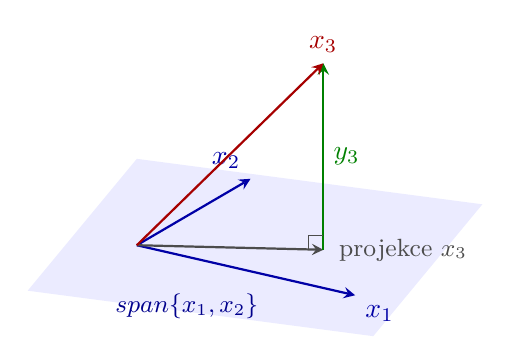
\begin{tikzpicture}[scale=1.155,>=stealth]
  \fill[blue!8] (-0.7,-0.45)--(3.1,-0.95)--(4.3,0.5)--(0.5,1.0)--cycle;
  \node[blue!55!black] at (1.05,-0.62) {\small$\spn\{x_1,x_2\}$};
  \coordinate (O)  at (0.5,0.05);
  \coordinate (x1) at (2.9,-0.5);
  \coordinate (x2) at (1.75,0.78);
  \coordinate (p)  at (2.55,0.0);
  \coordinate (x3) at (2.55,2.05);
  \draw[->,thick,blue!65!black] (O)--(x1) node[below right]{$x_1$};
  \draw[->,thick,blue!65!black] (O)--(x2) node[above left]{$x_2$};
  \draw[->,thick,gray!60!black] (O)--(p) node[pos=1,right=2pt]{\small projekce $x_3$};
  \draw[->,thick,green!50!black] (p)--(x3) node[midway,right]{$y_3$};
  \draw[->,thick,red!65!black]  (O)--(x3) node[above]{$x_3$};
  \draw[gray!60!black] ($(p)+(-0.16,0)$)--($(p)+(-0.16,0.16)$)--($(p)+(0,0.16)$);
\end{tikzpicture}
\obrpopis{Gram--Schmidt ve 3D: $y_3=x_3-\sum_{i=1}^{2}\frac{\langle x_3,z_i\rangle}{\langle z_i,z_i\rangle}z_i$ odečte projekci $x_3$ do roviny $\spn\{x_1,x_2\}$; pravý úhel u paty projekce ukazuje, že $y_3\perp x_1$ i $y_3\perp x_2$.}
\end{center}

\begin{priklad}[Gram--Schmidt]
\textbf{Zadání.} Ortonormalizujte $x_1=(1,0,1,0)^T$, $x_2=(1,1,1,1)^T$, $x_3=(1,0,0,1)^T$ (standardní součin).\par
\textbf{Řešení.}
\[
  z_1=\tfrac{\sqrt2}{2}(1,0,1,0)^T,\quad z_2=\tfrac{\sqrt2}{2}(0,1,0,1)^T,\quad z_3=\tfrac12(1,-1,-1,1)^T.
\]
\end{priklad}

\begin{priklad}[SZZ podzim 2022 č.~4: Báze a ortogonální báze sloupcového prostoru] \szzotazka{podzim 2022}{4}{Báze a ortogonální báze}\par
\textbf{Zadání.}
Buď $A=BC$, kde
\[
  B=\begin{pmatrix}1&3\\2&2\\1&2\\1&0\\1&-1\end{pmatrix}\ (5\times2),\qquad
  C=\begin{pmatrix}1&2&3&4&5\\5&4&3&2&1\end{pmatrix}\ (2\times5).
\]
(1) Najděte bázi sloupcového prostoru $A$. (2) Definujte pojem ortogonální báze. (3) Najděte ortogonální bázi sloupcového prostoru $A$.

\textbf{Řešení.}
\begin{enumerate}[label=(\arabic*)]
  \item Protože $C$ má plnou řádkovou hodnost $2$, je $\{Cx:x\in\mathbb{R}^5\}=\mathbb{R}^2$, takže $S(A)=\{B(Cx)\}=\{By:y\in\mathbb{R}^2\}=S(B)$ a~$\rank(A)=\rank(B)=2$. Bázi proto tvoří dva (lineárně nezávislé) sloupce $B$:
    \[ b_1=(1,2,1,1,1)^T,\qquad b_2=(3,2,2,0,-1)^T. \]
  \item \emph{Ortogonální báze} je báze, jejíž každé dva různé vektory mají nulový skalární součin (jsou na sebe kolmé).
  \item Gram--Schmidt na $b_1,b_2$: $u_1=b_1$, $\|u_1\|^2=8$, $b_2\cdot u_1=8$, tedy
    \[ u_2=b_2-\frac{b_2\cdot u_1}{\|u_1\|^2}\,u_1=b_2-\tfrac88\,u_1=(2,0,1,-1,-2)^T,\qquad u_1\cdot u_2=0. \]
    Hledaná ortogonální báze je $\{(1,2,1,1,1)^T,\ (2,0,1,-1,-2)^T\}$.
\end{enumerate}
\end{priklad}

\subsection{Ortogonální doplněk a projekce}

\begin{definice}[Ortogonální doplněk]
$M^\perp=\{x\in V;\ \langle x,y\rangle=0\ \forall y\in M\}$ je \emph{ortogonální doplněk} $M$; je to vždy podprostor a $M^\perp=\spn(M)^\perp$.
\end{definice}

\begin{veta}[Vlastnosti doplňku podprostoru]
Pro podprostor $U$ konečně generovaného $V$ platí $\dim V=\dim U+\dim U^\perp$, dále $V=U+U^\perp$, $U\cap U^\perp=\{o\}$ a $(U^\perp)^\perp=U$. (Rozšíříme-li ortonormální bázi $U$ na ortonormální bázi $V$, doplňkové vektory jsou ortonormální bází $U^\perp$.)
\end{veta}

\begin{definice}[Ortogonální projekce]
\emph{Projekcí} vektoru $x\in V$ do podprostoru $U$ je vektor $x_U\in U$ nejbližší k~$x$, tj. $\|x-x_U\|=\min_{y\in U}\|x-y\|$.
\end{definice}

\begin{veta}[O ortogonální projekci]
Projekce $x_U$ existuje a je jediná; je charakterizována tím, že $x-x_U\in U^\perp$. Je-li $z_1,\dots,z_m$ ortonormální báze $U$, pak
\[
  x_U=\sum_{i=1}^m\langle x,z_i\rangle z_i.
\]
Zobrazení $x\mapsto x_U$ je lineární (\emph{projekce jako lineární zobrazení}).
\end{veta}

\begin{center}
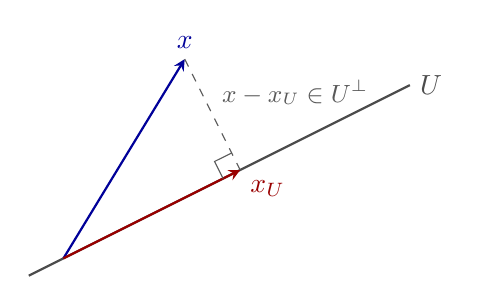
\begin{tikzpicture}[scale=1.1,>=stealth]
  \draw[thick,black!70] (-0.4,-0.2)--(4.0,2.0) node[right]{$U$};
  \coordinate (O) at (0,0);
  \coordinate (x) at (1.4,2.3);
  \coordinate (xu) at (2.04,1.02);
  \draw[->,thick,blue!60!black] (O)--(x) node[above]{$x$};
  \draw[->,thick,red!60!black] (O)--(xu) node[below right]{$x_U$};
  \draw[dashed,gray!70!black] (x)--(xu) node[midway,above right]{\small$x-x_U\in U^\perp$};
  \draw[gray!70!black] ($(xu)+(-0.098,0.197)$)--($(xu)+(-0.295,0.099)$)--($(xu)+(-0.197,-0.098)$);
\end{tikzpicture}
\obrpopis{Ortogonální projekce: $x_U=\arg\min_{u\in U}\|x-u\|$ je nejbližší bod $U$, rozdíl $x-x_U$ kolmý na $U$ (pravý úhel u paty); pro přímku $U=\spn\{a\}$ je $x_U=\frac{x^Ta}{a^Ta}\,a$.}
\end{center}

\begin{priklad}[Projekce na přímku]
Projekce $x\in\mathbb{R}^n$ na přímku $\spn\{a\}$ ($a\neq o$) je $x_U=\dfrac{x^Ta}{a^Ta}\,a$. Pro $U$ s~bází $w_1,\dots,w_m$ bez ortonormalizace dostaneme souřadnice projekce řešením soustavy $G\,[x_U]_B=(\langle w_1,x\rangle,\dots,\langle w_m,x\rangle)^T$ s~regulární \emph{Gramovou maticí} $G_{ij}=\langle w_i,w_j\rangle$.
\end{priklad}

\video{https://www.youtube.com/watch?v=LyGKycYT2v0}{3Blue1Brown, \emph{Essence of Linear Algebra} kap.~9 -- \emph{Dot products and duality} (skalární součin a~projekce).}

\subsection{Ortogonální matice}

\begin{definice}[Ortogonální matice]
$Q\in\mathbb{R}^{n\times n}$ je \emph{ortogonální}, pokud $Q^TQ=I_n$.
\end{definice}

\begin{veta}[Charakterizace a vlastnosti]
Pro $Q\in\mathbb{R}^{n\times n}$ jsou ekvivalentní:
\begin{enumerate}[label=(\arabic*)]
  \item $Q$ je ortogonální;
  \item $Q^{-1}=Q^T$;
  \item $QQ^T=I_n$;
  \item sloupce (resp.\ řádky) $Q$ tvoří ortonormální bázi $\mathbb{R}^n$.
\end{enumerate}
Ortogonální matice navíc \emph{zachovává skalární součin i~normu}: $\langle Qx,Qy\rangle=\langle x,y\rangle$ a~$\|Qx\|=\|x\|$. Součin ortogonálních matic je opět ortogonální.
\end{veta}

\begin{intuice}
Ortogonální matice je matice zobrazení, které nedeformuje objekty -- zachovává délky a úhly. Geometricky jde o složení rotací a zrcadlení. Každá ortogonální matice řádu~2 je buď rotace $\begin{psmallmatrix}\cos\varphi&-\sin\varphi\\\sin\varphi&\cos\varphi\end{psmallmatrix}$, nebo rotace složená s~překlopením.
\end{intuice}

\begin{priklad}[SZZ jaro 2024 č.~3: Skalární součin na maticích] \szzotazka{jaro 2024}{3}{Skalární součin}\par
\textbf{Zadání.}
\begin{enumerate}[label=(\arabic*)]
  \item Ověřte, že $\langle A,B\rangle=\tr(A^TB)$ je skalární součin na $\mathbb{R}^{m\times n}$, kde $\tr(C)=\sum_i c_{ii}$.
  \item Rozhodněte, zda jsou matice $A\in\mathbb{R}^{4\times6}$ s~prvky rostoucími po antidiagonálách (řádky $(1,-2,3,-4,5,-6)$, $(-2,3,\dots)$, \dots) a~matice $B$ se všemi prvky $-13$ \emph{na sebe ortogonální} vzhledem k~tomuto skalárnímu součinu (tj.\ zda $\langle A,B\rangle=0$).
  \item Zformulujte CS nerovnost a~rozhodněte, zda pro čtvercovou $A$ řádu~$n$ platí $(\tr A)^2\le n\cdot\tr(A^TA)$.
\end{enumerate}

\textbf{Řešení.}
\begin{enumerate}[label=(\arabic*)]
  \item Rozepsáním $\tr(A^TB)=\sum_{i,j}a_{ij}b_{ij}$ -- to je standardní skalární součin, díváme-li se na matici $m\times n$ jako na vektor o~$mn$ složkách. Axiomy se ověří přímo: $\langle A,A\rangle=\sum_{i,j}a_{ij}^2\ge0$ s~rovností jen pro $A=0$; symetrie i~linearita jsou zřejmé.
  \item $\langle A,B\rangle=\sum_{i,j}a_{ij}\cdot(-13)=-13\sum_{i,j}a_{ij}$. Součet všech prvků $A$ je součet jejích řádkových součtů $-3+3-3+3=0$, takže $\langle A,B\rangle=0$ -- matice \emph{jsou} na sebe ortogonální.
  \item CS nerovnost: $|\langle u,v\rangle|\le\|u\|\,\|v\|$, po umocnění $\langle u,v\rangle^2\le\langle u,u\rangle\langle v,v\rangle$. Nerovnost srovnává $(\tr A)^2$ s~$n\cdot\tr(A^TA)$; protože $\tr A=\langle I_n,A\rangle$, volíme v~CS $u=I_n$, $v=A$:
    \[ \langle I_n,A\rangle=\tr(I_n^TA)=\tr A,\qquad \langle I_n,I_n\rangle=\tr(I_n)=n,\qquad \langle A,A\rangle=\tr(A^TA). \]
    Dosazením do CS dostáváme $(\tr A)^2\le n\cdot\tr(A^TA)$ -- nerovnost \emph{platí}.
\end{enumerate}
\end{priklad}

% ============================================================
\section{Determinanty (Laplaceův rozvoj, geometrie)}

\subsection{Definice a základní vlastnosti}

\begin{definice}[Determinant]
Pro $A\in T^{n\times n}$ je
\[
  \det(A)=\sum_{p\in S_n}\sgn(p)\,a_{1,p(1)}a_{2,p(2)}\cdots a_{n,p(n)}.
\]
\end{definice}

\begin{intuice}
Každý sčítanec vybere z matice $n$ prvků tak, že z~každého řádku a~každého sloupce právě jeden, vynásobí je a opatří znaménkem permutace. Pro $n=2$: $\det\begin{psmallmatrix}a&b\\c&d\end{psmallmatrix}=ad-bc$; pro $n=3$ Sarrusovo pravidlo (šest členů).
\end{intuice}

\begin{veta}[Základní vlastnosti]
\begin{itemize}
  \item $\det(A^T)=\det(A)$;
  \item determinant trojúhelníkové matice je součin prvků na diagonále (speciálně $\det I_n=1$);
  \item \emph{multiplikativnost}: $\det(AB)=\det(A)\det(B)$, a~tedy $\det(A^{-1})=\det(A)^{-1}$;
  \item vliv ERÚ: vynásobení řádku číslem $\alpha$ násobí determinant $\alpha$; výměna dvou řádků mění znaménko; přičtení násobku řádku k~jinému determinant nemění;
  \item má-li matice dva stejné (nebo nulový) řádky, je $\det(A)=0$.
\end{itemize}
\end{veta}

\begin{veta}[Kritérium regularity a vztah s vlastními čísly]
$A\in T^{n\times n}$ je regulární právě tehdy, když $\det(A)\neq0$. Navíc $\det(A)$ je roven součinu vlastních čísel matice $A$ (viz sekci~8).
\end{veta}

\begin{poznamka}[Výpočet determinantu Gaussovou eliminací]
Z vlivu ERÚ plyne praktický postup: převedeme $A$ na REF (horní trojúhelníkový tvar), zapamatujeme si změny determinantu (znaménko a škálování), a $\det(A)$ je součin diagonálních prvků poděleno nasbíraným faktorem.
\end{poznamka}

\begin{veta}[Laplaceův rozvoj]
Pro $n\ge2$ a libovolné $i$ platí (rozvoj podle $i$-tého řádku; analogicky podle sloupce)
\[
  \det(A)=\sum_{j=1}^n(-1)^{i+j}a_{ij}\det(A_{ij}),
\]
kde $A_{ij}$ vznikne z $A$ vyškrtnutím $i$-tého řádku a $j$-tého sloupce.
\end{veta}

\begin{priklad}[Laplaceův rozvoj]
\textbf{Zadání.} Spočítejte $\det\begin{psmallmatrix}2&1&0\\1&3&1\\0&1&2\end{psmallmatrix}$ Laplaceovým rozvojem.\par
\textbf{Řešení.} Rozvineme podle 1.\ řádku: pro každý prvek $a_{1j}$ vezmeme jeho \emph{minor} (determinant matice po vyškrtnutí 1.\ řádku a~$j$-tého sloupce) se znaménkem $(-1)^{1+j}$:
\[
  \det A=+\,2\cdot\det\begin{psmallmatrix}3&1\\1&2\end{psmallmatrix}\;-\;1\cdot\det\begin{psmallmatrix}1&1\\0&2\end{psmallmatrix}\;+\;0\cdot\det\begin{psmallmatrix}1&3\\0&1\end{psmallmatrix}
  =2(6-1)-1(2-0)+0=8.
\]
Rozvíjet se vyplatí podle řádku či sloupce s~nejvíce nulami. U~velkých matic je efektivnější převést matici na trojúhelníkový tvar Gaussovou eliminací (s~hlídáním faktorů) a~determinant odečíst jako součin diagonály.
\end{priklad}

\subsection{Geometrická interpretace}

\begin{veta}[Determinant jako objem]
Zobrazení $x\mapsto Ax$ s $A\in\mathbb{R}^{n\times n}$ mění objem geometrických těles s~koeficientem $|\det(A)|$. Speciálně objem rovnoběžnostěnu napjatého na řádky (resp.\ sloupce) matice $A$ je $|\det(A)|$. Znaménko $\det(A)$ udává orientaci (pravo-/levotočivost).
\end{veta}

\begin{center}
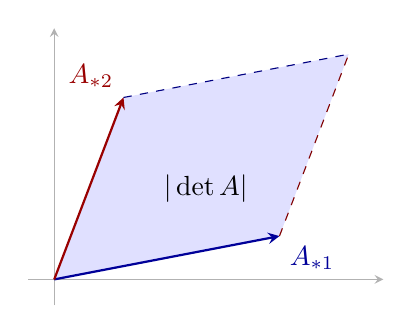
\begin{tikzpicture}[scale=1.1,>=stealth]
  \draw[->,gray!60] (-0.3,0)--(3.8,0);
  \draw[->,gray!60] (0,-0.3)--(0,2.9);
  \coordinate (O) at (0,0);
  \coordinate (a) at (2.6,0.5);
  \coordinate (b) at (0.8,2.1);
  \fill[blue!12] (O)--(a)--($(a)+(b)$)--(b)--cycle;
  \draw[->,thick,blue!60!black] (O)--(a) node[below right]{$A_{*1}$};
  \draw[->,thick,red!60!black] (O)--(b) node[above left]{$A_{*2}$};
  \draw[blue!50!black,dashed] (b)--($(a)+(b)$);
  \draw[red!50!black,dashed] (a)--($(a)+(b)$);
  \node at (1.75,1.05){$|\det A|$};
\end{tikzpicture}
\obrpopis{V $\mathbb{R}^2$ je $|\det A|=|a_{11}a_{22}-a_{12}a_{21}|$ obsah rovnoběžníku napjatého na sloupce $A_{*1},A_{*2}$ (např. pro $A_{*1}=(2{,}6;\,0{,}5)$, $A_{*2}=(0{,}8;\,2{,}1)$ vyjde obsah $|2{,}6\cdot 2{,}1-0{,}5\cdot 0{,}8|=5{,}06$).}
\end{center}

\video{https://www.youtube.com/watch?v=Ip3X9LOh2dk}{3Blue1Brown, \emph{Essence of Linear Algebra} kap.~6 -- \emph{The determinant} (determinant jako faktor změny objemu a~orientace).}

\video{https://www.youtube.com/watch?v=jBsC34PxzoM}{3Blue1Brown, \emph{Essence of Linear Algebra} kap.~12 -- \emph{Cramer's rule, explained geometrically} (Cramerovo pravidlo geometricky, přes objemy/determinanty).}

\begin{priklad}[SZZ jaro 2026 č.~3: Hodnost, determinant, ortogonální báze jádra] \szzotazka{jaro 2026}{3}{Matice}\par
\textbf{Zadání.}
Buď $A\in\mathbb{R}^{3\times3}$, jejíž řádkový prostor má bázi tvořenou pouze vektorem $(1,2,3)^T$.
\begin{enumerate}[label=(\arabic*)]
  \item Najděte odstupňovaný tvar $A$.
  \item Napište definici determinantu a~spočítejte $\det(A)$.
  \item Najděte ortogonální bázi jádra $A$.
\end{enumerate}

\textbf{Řešení.}
\begin{enumerate}[label=(\arabic*)]
  \item Všechny řádky jsou násobky $(1,2,3)$, tedy $\rank(A)=1$ a~odstupňovaný tvar je $\begin{psmallmatrix}1&2&3\\0&0&0\\0&0&0\end{psmallmatrix}$.
  \item Definice viz výše. Protože $\rank(A)=1<3$, je $A$ singulární, takže $\det(A)=0$.
  \item \textbf{Báze jádra.} $\Ker(A)=\{x:(1,2,3)\cdot x=0\}$ má dimenzi $3-1=2$; bázi tvoří např.\ $(2,-1,0)^T$ a~$(3,0,-1)^T$.\par
    \textbf{Gram--Schmidt.}
    \[
    \begin{aligned}
      y_1&=(2,-1,0)^T,\\
      y_2&=(3,0,-1)^T-\frac{(3,0,-1)\cdot(2,-1,0)}{(2,-1,0)\cdot(2,-1,0)}\,(2,-1,0)^T=(3,0,-1)^T-\tfrac65(2,-1,0)^T=\tfrac15(3,6,-5)^T.
    \end{aligned}
    \]
    Ortogonální báze jádra je tedy $\boxed{(2,-1,0)^T,\ \ (3,6,-5)^T}$.
\end{enumerate}
\end{priklad}

\begin{priklad}[SZZ léto 2023 č.~3: Kolmost, zobrazení, změna obsahu] \szzotazka{léto 2023}{3}{Lineární algebra}\par
\textbf{Zadání.}
Pro $A=\begin{psmallmatrix}1&2\\1&1\end{psmallmatrix}$ a~$B=\begin{psmallmatrix}0&1\\1&2\end{psmallmatrix}$:
\begin{enumerate}[label=(\arabic*)]
  \item najděte $x\in\mathbb{R}^2$ tak, aby $Ax\perp Bx$ (standardní součin);
  \item najděte matici zobrazení, které $Ax$ posílá na $Bx$ pro všechna $x$;
  \item rozhodněte, zda zobrazení $x\mapsto B^{-1}A^3B^{-1}x$ obsahy útvarů zvětšuje či zmenšuje.
\end{enumerate}

\textbf{Řešení.}
\begin{enumerate}[label=(\arabic*)]
  \item $Ax=(x_1+2x_2,\,x_1+x_2)^T$ a~$Bx=(x_2,\,x_1+2x_2)^T$. Jejich skalární součin je
    \[ (x_1+2x_2)\,x_2+(x_1+x_2)(x_1+2x_2)=(x_1+2x_2)(x_2+x_1+x_2)=(x_1+2x_2)^2, \]
    což je nula právě tehdy, když $x_1+2x_2=0$, tj.\ $\boxed{x=t(-2,1)^T,\ t\in\mathbb{R}}$.
  \item Hledáme $M$ s~$M(Ax)=Bx$ pro všechna $x$. Protože $A$ je regulární ($\det A=-1$), prochází $Ax$ celé $\mathbb{R}^2$, takže podmínka je $MA=B$, odkud $M=BA^{-1}$. Z~$A^{-1}=\begin{psmallmatrix}-1&2\\1&-1\end{psmallmatrix}$ dostaneme
    \[ M=BA^{-1}=\begin{pmatrix}0&1\\1&2\end{pmatrix}\begin{pmatrix}-1&2\\1&-1\end{pmatrix}=\begin{pmatrix}1&-1\\1&0\end{pmatrix}\qquad(\text{ověření }MA=B). \]
  \item Faktor změny obsahu je $|\det(B^{-1}A^3B^{-1})|=\dfrac{|\det A|^3}{|\det B|^2}$. Zde $\det A=-1$ a~$\det B=-1$, takže faktor je $\boxed{\tfrac{1}{1}=1}$: obsahy se \emph{nemění} (zobrazení je zachovává, jen převrací orientaci, neboť celkový determinant je $-1<0$).
\end{enumerate}
\end{priklad}

% ============================================================
\section{Vlastní čísla a vektory (diagonalizace, spektrální rozklad)}

\subsection{Vlastní čísla a charakteristický polynom}

\begin{definice}[Vlastní číslo a vektor]
Číslo $\lambda\in\mathbb{C}$ je \emph{vlastním číslem} matice $A\in\mathbb{C}^{n\times n}$, existuje-li nenulový \emph{vlastní vektor} $x$ s $Ax=\lambda x$.
\end{definice}

\begin{veta}[Charakterizace]
$\lambda$ je vlastním číslem $A$ právě tehdy, když $\det(A-\lambda I_n)=0$; příslušné vlastní vektory jsou nenulové prvky $\Ker(A-\lambda I_n)$.
\end{veta}

\begin{definice}[Charakteristický polynom, násobnosti]
$p_A(\lambda)=\det(A-\lambda I_n)$ je \emph{charakteristický polynom} (stupně $n$). \emph{Algebraická násobnost} $\lambda$ je jeho násobnost jako kořene $p_A$; \emph{geometrická násobnost} je $n-\rank(A-\lambda I_n)$ (počet lineárně nezávislých vlastních vektorů). Vždy platí geometrická $\le$ algebraická.
\end{definice}

\begin{intuice}
Vlastní vektor je \uv{invariantní směr}: zobrazení $x\mapsto Ax$ ho jen natáhne (faktorem $\lambda$), neotočí. Vlastní čísla najdeme jako kořeny $p_A$, vlastní vektory pak jako jádro $A-\lambda I_n$.
\end{intuice}

\begin{center}
\begin{tikzpicture}[scale=1.045,>=stealth]
  \draw[->,gray!55] (-2.6,0)--(2.8,0);
  \draw[->,gray!55] (0,-1.6)--(0,2.6);
  \coordinate (O) at (0,0);
  % eigen direction along (1,1): v and Av=2v
  \draw[gray!40,dash pattern=on2pt off2pt] (-1.6,-1.6)--(2.2,2.2);
  \draw[->,thick,blue!60!black] (O)--(1,1) node[above left]{$v$};
  \draw[->,thick,blue!40!black] (O)--(2,2) node[right]{$Av=\lambda v$};
  % non-eigen vector w rotates
  \draw[->,thick,red!60!black] (O)--(1.4,-0.4) node[below]{$w$};
  \draw[->,thick,red!35!black] (O)--(0.6,1.2) node[above]{$Aw$};
\end{tikzpicture}
\obrpopis{Vlastní vektor $v=(1,1)^T$ pro $\lambda=2$: zůstává na své přímce, jen se škáluje ($Av=2v$). Obecný vektor $w=(1{,}4;\,-0{,}4)^T$ se otočí mimo svůj směr ($Aw$ na něm neleží).}
\end{center}

\video{https://www.youtube.com/watch?v=PFDu9oVAE-g}{3Blue1Brown, \emph{Essence of Linear Algebra} kap.~14 -- \emph{Eigenvectors and eigenvalues} (vlastní směry a~faktory).}

\begin{veta}[Stopa a determinant ze spektra]
Má-li $A\in\mathbb{C}^{n\times n}$ vlastní čísla $\lambda_1,\dots,\lambda_n$ (včetně násobností), pak $\det(A)=\lambda_1\cdots\lambda_n$ a $\tr(A)=\lambda_1+\dots+\lambda_n$. (U reálné matice se komplexní vlastní čísla vyskytují v~komplexně sdružených párech.)
\end{veta}

\video{https://www.youtube.com/watch?v=e50Bj7jn9IQ}{3Blue1Brown, \emph{Essence of Linear Algebra} kap.~15 -- \emph{A quick trick for computing eigenvalues} (rychlý výpočet vlastních čísel $2\times2$ ze stopy a~determinantu -- viz vztah výše).}

\subsection{Podobnost a diagonalizovatelnost}

\begin{definice}[Podobnost]
$A,B\in\mathbb{C}^{n\times n}$ jsou \emph{podobné}, existuje-li regulární $S$ s $A=SBS^{-1}$.
\end{definice}

\begin{veta}[Podobné matice]
Podobné matice mají stejný charakteristický polynom, tedy stejná vlastní čísla (i násobnosti), stejnou hodnost i determinant. Vlastní vektory se obecně liší.
\end{veta}

\begin{intuice}
Podobnost = táž lineární transformace v~jiné bázi ($S$ je matice přechodu). Proto se vlastní čísla nemění -- jsou vlastností zobrazení, ne souřadnic. Naopak jádro se měnit může: $\begin{psmallmatrix}1&0\\0&0\end{psmallmatrix}$ a $\begin{psmallmatrix}0&0\\0&1\end{psmallmatrix}$ jsou podobné, ale mají různá jádra.
\end{intuice}

\video{https://www.youtube.com/watch?v=P2LTAUO1TdA}{3Blue1Brown, \emph{Essence of Linear Algebra} kap.~13 -- \emph{Change of basis} (změna báze).}

\begin{definice}[Diagonalizovatelnost a spektrální rozklad]
$A$ je \emph{diagonalizovatelná}, je-li podobná diagonální matici, tj.\ $A=S\Lambda S^{-1}$ se $\Lambda$ diagonální. Tomuto rozkladu se říká \emph{spektrální rozklad} (na diagonále $\Lambda$ je spektrum).
\end{definice}

\begin{veta}[Charakterizace diagonalizovatelnosti]
$A\in\mathbb{C}^{n\times n}$ je diagonalizovatelná právě tehdy, když má $n$ lineárně nezávislých vlastních vektorů; ty pak tvoří sloupce $S$ a příslušná vlastní čísla diagonálu $\Lambda$. Ekvivalentně: pro každé vlastní číslo splývá algebraická a geometrická násobnost. Speciálně má-li $A$ $n$ navzájem různých vlastních čísel, je diagonalizovatelná.
\end{veta}

\begin{poznamka}[Mocniny matice]
Diagonalizace usnadňuje mocnění: $A^k=S\Lambda^kS^{-1}$, kde $\Lambda^k$ jen umocní diagonálu. Toho se využívá k řešení rekurencí (Fibonacci) či studiu asymptotiky.
\end{poznamka}

\subsection{Symetrické matice}

Reálné symetrické matice ($A=A^T$) se chovají obzvlášť hezky: vlastní čísla jsou vždy reálná a vlastní vektory lze vybrat navzájem kolmé. To z~nich dělá nejdůležitější diagonalizovatelnou třídu (váže se např.\ na kovarianční matice a PCA ve strojovém učení).

\begin{veta}[Spektrální rozklad symetrické matice]
Reálná symetrická matice $A\in\mathbb{R}^{n\times n}$ má vždy reálná vlastní čísla a je \emph{ortogonálně diagonalizovatelná}: existuje ortogonální $Q$ a diagonální $\Lambda$ tak, že $A=Q\Lambda Q^T$. Vlastní vektory příslušné různým vlastním číslům jsou na sebe kolmé, takže lze vybrat ortonormální bázi z~vlastních vektorů.
\end{veta}

\begin{intuice}
Symetrická matice odpovídá \uv{samosdruženému} zobrazení ($\langle Ax,y\rangle=\langle x,Ay\rangle$); to vynutí, že různým vlastním číslům příslušejí kolmé vlastní vektory. V~bázi z~těchto vlastních vektorů je zobrazení čistě \uv{škálování podél kolmých os}, proto $A=Q\Lambda Q^T$ s~ortogonální $Q$.
\end{intuice}

\begin{priklad}[SZZ jaro 2025 č.~3: Symetrická matice, podobnost, diagonalizace] \szzotazka{jaro 2025}{3}{Matice}\par
\textbf{Zadání.}
\begin{enumerate}[label=(\arabic*)]
  \item Najděte symetrickou $S\in\mathbb{R}^{3\times3}$ s~$\Ker(S)=\spn\{(1,5,1)^T,(0,2,1)^T\}$.
  \item Definujte podobné matice a~uveďte, které z~veličin hodnost / determinant / jádro mají podobné matice stejné.
  \item Matice $A=\begin{psmallmatrix}2&2&3\\0&-1&-4\\1&2&4\end{psmallmatrix}$ má vlastní čísla $3$ a~$1$. Je diagonalizovatelná?
\end{enumerate}

\textbf{Řešení.}
\begin{enumerate}[label=(\arabic*)]
  \item \textbf{Kolmost na jádro.} Pro symetrickou $S$ je řádkový prostor roven sloupcovému a~kolmý na jádro (neboť $S(S)^\perp=\Ker(S^T)=\Ker(S)$). Jádro je 2-rozměrné, takže řádkový prostor je 1-rozměrný, generovaný vektorem kolmým na oba vektory jádra:
    \[ (1,5,1)\times(0,2,1)=(3,-1,2). \]
    \textbf{Konstrukce.} Symetrická matice hodnosti~1 s~tímto řádkovým prostorem je
    \[ S=\alpha\,(3,-1,2)^T(3,-1,2)=\alpha\begin{pmatrix}9&-3&6\\-3&1&-2\\6&-2&4\end{pmatrix},\qquad \alpha\neq0. \]
    (Ověření: $(3,-1,2)$ je kolmý na oba generátory jádra, takže $Sx=o$ pro $x$ z~jádra.)
  \item $A,B$ jsou podobné, je-li $A=RBR^{-1}$ pro regulární $R$. Stejné mají \emph{hodnost} i~\emph{determinant}; \emph{jádro} obecně ne (protipříklad $\begin{psmallmatrix}1&0\\0&0\end{psmallmatrix}$ a~$\begin{psmallmatrix}0&0\\0&1\end{psmallmatrix}$).
  \item \textbf{Třetí vlastní číslo ze stopy.} Stopa je $2-1+4=5=3+1+\lambda_3$, takže $\lambda_3=1$ -- číslo $1$ je dvojnásobné (algebraicky).\par
    \textbf{Algebraická vs. geometrická.} $\rank(A-I_3)=2$, takže geometrická násobnost čísla $1$ je $3-2=1<2$. Násobnosti nesplývají, takže $\boxed{A\text{ není diagonalizovatelná}}$.
\end{enumerate}
\end{priklad}

\begin{priklad}[SZZ léto 2024 č.~3: Steinitz a výměna vlastních vektorů] \szzotazka{léto 2024}{3}{Báze vektorových prostorů}\par
\textbf{Zadání.}
\begin{enumerate}[label=(\arabic*)]
  \item Zformulujte Steinitzovu větu o~výměně.
  \item Reálná $A$ je diagonalizovatelná jako $D=R^{-1}AR$ s~diagonálou $D=(17,17,23,17,23)$, kde vlastní vektory tvoří sloupce
    \[
      R=\begin{pmatrix}
        -1 & -1 & -8 & -2 & -8\\
        0 & 1 & -3 & 0 & 2\\
        -1 & -2 & 6 & -2 & 3\\
        -1 & -3 & 7 & -1 & -4\\
        1 & 2 & 0 & 2 & 4
      \end{pmatrix}.
    \]
    Rozhodněte, zda lze některý sloupec $R$ vyměnit za vektor $u_i$ tak, aby $A$ šla diagonalizovat i~výslednou maticí $R'$: \ (a)~$u_1=(4,2,2,-3,-2)^T$; \ (b)~$u_2=(7,-6,-2,12,-6)^T$.
\end{enumerate}

\textbf{Řešení.}
\begin{enumerate}[label=(\arabic*)]
  \item Viz znění Steinitzovy věty v~sekci~4.
  \item Sloupce $R$ jsou vlastní vektory; podle diagonály patří sloupce $1,2,4$ vlastnímu číslu $17$ (vlastní podprostor dimenze~3) a~sloupce $3,5$ vlastnímu číslu $23$. Aby $R'$ stále diagonalizovala $A$, musí být nový sloupec opět vlastním vektorem a~výsledek musí být báze.
    \begin{itemize}
      \item[(a)] $[u_1]_B=(0,2,0,-3,0)^T$, tedy $u_1=2R_{*2}-3R_{*4}$. Oba leží v~podprostoru čísla $17$, takže $u_1$ je vlastní vektor pro $17$. Vyměnit lze ty sloupce s~nenulovým koeficientem, po nichž zůstane báze -- tedy sloupec~2 nebo sloupec~4.
      \item[(b)] $[u_2]_B=(0,1,1,0,-2)^T$, tj.\ $u_2=R_{*2}+R_{*3}-2R_{*5}$ míchá vlastní podprostory čísel $17$ a~$23$. Vektor $u_2$ proto není vlastním vektorem a~výměnu provést \emph{nelze}.
    \end{itemize}
\end{enumerate}
\end{priklad}

% ============================================================
\section{Pozitivně (semi)definitní matice (Choleského rozklad)}

\begin{definice}[Pozitivně (semi)definitní matice]
Symetrická $A\in\mathbb{R}^{n\times n}$ je \emph{pozitivně definitní}, pokud $x^TAx>0$ pro každé $x\neq o$, a \emph{pozitivně semidefinitní}, pokud $x^TAx\ge0$ pro každé $x$.
\end{definice}

\begin{veta}[Charakterizace pozitivní definitnosti]
Pro symetrickou $A\in\mathbb{R}^{n\times n}$ je ekvivalentní:
\begin{enumerate}[label=(\arabic*)]
  \item $A$ je pozitivně definitní;
  \item všechna vlastní čísla $A$ jsou kladná;
  \item existuje $U$ hodnosti $n$ s $A=U^TU$.
\end{enumerate}
(Pro semidefinitnost: vlastní čísla nezáporná, resp.\ $A=U^TU$ pro nějaké $U$.) Je-li $A$ pozitivně definitní, je regulární a $A^{-1}$ je rovněž pozitivně definitní.
\end{veta}

\begin{intuice}
Pozitivní definitnost znamená, že kvadratická forma $x^TAx$ je \uv{miskovitá} -- má v~počátku ostré minimum. Protože $\det(A)=\prod\lambda_i$, je u~pozitivně definitní matice determinant kladný; obráceně to ale samo o sobě nestačí (nutno více podmínek -- viz Sylvester).
\end{intuice}

\begin{veta}[Vztah se skalárním součinem]
Operace $\langle x,y\rangle=x^TAy$ je skalárním součinem na $\mathbb{R}^n$ právě tehdy, když $A$ je pozitivně definitní. (Tím jsou popsány všechny skalární součiny na $\mathbb{R}^n$.)
\end{veta}

\begin{veta}[Sylvestrovo kritérium]
Symetrická $A$ je pozitivně definitní právě tehdy, když všechny \emph{hlavní vedoucí minory} (determinanty levých horních podmatic $A_1,\dots,A_n$) jsou kladné.
\end{veta}

\begin{poznamka}[Testování Gaussovou eliminací]
Symetrická $A$ je pozitivně definitní právě tehdy, když ji Gaussova eliminace (jen přičítání násobků řádku s~pivotem k~řádkům pod ním) převede na tvar s~kladnou diagonálou. To je výpočetně levnější než Sylvestrovo kritérium.
\end{poznamka}

\begin{veta}[Choleského rozklad]
Pro každou pozitivně definitní $A\in\mathbb{R}^{n\times n}$ existuje \emph{jediná} dolní trojúhelníková matice $L$ s~kladnou diagonálou taková, že
\[
  A=LL^T.
\]
\end{veta}

\begin{intuice}
Choleský je \uv{odmocnina} pozitivně definitní matice ve tvaru trojúhelníkového činitele. Je to nejúčinnější test pozitivní definitnosti (řádově $\tfrac13n^3$ operací) a zároveň praktický nástroj pro řešení soustav $Ax=b$ s~pozitivně definitní $A$ (přes $Ly=b$ a $L^Tx=y$) a pro jejich inverzi.
\end{intuice}

\begin{priklad}[Výpočet Choleského rozkladu]
\textbf{Zadání.} Najděte Choleského rozklad $A=LL^T$ pozitivně definitní matice $A=\begin{psmallmatrix}4&-2&4\\-2&10&1\\4&1&6\end{psmallmatrix}$.\par
\textbf{Řešení.} Prvky dolní trojúhelníkové $L$ určíme porovnáním $A=LL^T$ po sloupcích shora dolů:
\[
\begin{aligned}
  \ell_{11}&=\sqrt{a_{11}}=\sqrt4=2, & \ell_{21}&=\tfrac{a_{21}}{\ell_{11}}=\tfrac{-2}{2}=-1, & \ell_{31}&=\tfrac{a_{31}}{\ell_{11}}=\tfrac{4}{2}=2,\\
  \ell_{22}&=\sqrt{a_{22}-\ell_{21}^2}=\sqrt{10-1}=3, & \ell_{32}&=\tfrac{a_{32}-\ell_{31}\ell_{21}}{\ell_{22}}=\tfrac{1-2\cdot(-1)}{3}=1, &&\\
  \ell_{33}&=\sqrt{a_{33}-\ell_{31}^2-\ell_{32}^2}=\sqrt{6-4-1}=1. &&&&
\end{aligned}
\]
Tedy $\boxed{L=\begin{psmallmatrix}2&0&0\\-1&3&0\\2&1&1\end{psmallmatrix}}$ (snadno ověříme $LL^T=A$). Kdyby pod některou odmocninou vyšlo nekladné číslo, matice by nebyla pozitivně definitní.
\end{priklad}

\begin{priklad}[SZZ léto 2025 č.~3: Skalární součin $x^TAy$ a pozitivní definitnost] \szzotazka{léto 2025}{3}{Skalární součin}\par
\textbf{Zadání.}
Uvažujme $\langle x,y\rangle=x^TAy$ pro symetrickou $A$.
\begin{enumerate}[label=(\arabic*)]
  \item Rozhodněte: \ (a)~je-li $x^TAy$ skalární součin, je $\det(A)>0$? \ (b)~je-li $B$ symetrická regulární, je $x^TB^2y$ skalární součin?
  \item Zapište CS nerovnost pro $\langle x,y\rangle=x^TAy$ pomocí maticových operací.
  \item Je matice $A$ s~prvky $a_{ij}=\min(i,j)$ pozitivně definitní pro všechna $n\ge1$? Formulujte kritérium a~ověřte.
\end{enumerate}
\textbf{Řešení.}
\begin{enumerate}[label=(\arabic*)]
  \item \begin{itemize}
      \item[(a)] \emph{Ano}: skalární součin $\Rightarrow$ $A$ pozitivně definitní $\Rightarrow$ kladná vlastní čísla $\Rightarrow$ $\det(A)=\prod\lambda_i>0$.
      \item[(b)] \emph{Ano}: $B^2=B^TB$ je symetrická a~její vlastní čísla jsou $(\lambda_i^B)^2>0$ (regulární $B$ nemá nulové vlastní číslo), takže $B^2$ je pozitivně definitní a~$x^TB^2y$ je skalární součin.
    \end{itemize}
  \item CS $|\langle x,y\rangle|\le\|x\|\,\|y\|$ má zde tvar $|x^TAy|\le\sqrt{x^TAx}\,\sqrt{y^TAy}$.
  \item \textbf{Kritérium.} Symetrická matice je pozitivně definitní, má-li Choleského rozklad $A=LL^T$ (ekvivalentně kladná vlastní čísla / kladné hlavní vedoucí minory).\par
    \textbf{Konstrukce $L$.} Pro $a_{ij}=\min(i,j)$ vezmeme dolní trojúhelníkovou $L$ se samými jedničkami (v~dolní části i~na diagonále). Pak
    \[ (LL^T)_{ij}=\sum_k L_{ik}L_{jk}=\#\{k:k\le i\text{ a }k\le j\}=\min(i,j)=a_{ij}. \]
    Tedy $A=LL^T$ existuje a~$\boxed{A\text{ je p.d.\ pro všechna }n\ge1}$.
\end{enumerate}
\end{priklad}

% ============================================================
\section*{Shrnutí}
\addcontentsline{toc}{section}{Shrnutí}

\begin{poznamka}
\textbf{Klíčové vlastnosti a vzorce (přehled k~SZZ).} Stručný výčet klíčových definic, vět a vzorců okruhu M2. Zkratky: LN $=$ lineárně nezávislé, LZ $=$ lineárně závislé, p.d.\ $=$ pozitivně definitní, psd $=$ pozitivně semidefinitní.

\smallskip
\emph{Algebra (grupy, permutace, tělesa).}
\begin{itemize}
  \item Grupa: asociativita, neutrální prvek, ke~každému prvku inverze; \emph{podgrupa} $=$ neprázdná podmnožina uzavřená na operaci i~inverzi. Komutativní grupa $=$ abelovská.
  \item Permutace: $\sgn(\pi)=(-1)^{\#\text{transpozic}}=(-1)^{n-\#\text{cyklů}}$; $\sgn(\pi\sigma)=\sgn(\pi)\sgn(\sigma)$; sudá vs.\ lichá.
  \item Těleso: $\mathbb{Z}_p$ je těleso $\iff p$ je prvočíslo; inverze v~$\mathbb{Z}_p$ přes malou Fermatovu větu ($a^{p-1}=1$, tedy $a^{-1}=a^{p-2}$). Konečné těleso má $p^k$ prvků.
\end{itemize}

\smallskip
\emph{Soustavy, matice, hodnost.}
\begin{itemize}
  \item Frobenius: $Ax=b$ řešitelná $\iff\rank(A)=\rank(A\,|\,b)$; právě jedno řešení $\iff$ navíc $\rank=n$ (počet neznámých), více řešení $\iff\rank<n$ (nad $\mathbb{R}$ nekonečně mnoho, nad $\mathbb{Z}_p$ jich je $p^{\,n-r}$). Množina řešení $=$ partikulární řešení $+\,\Ker(A)$ (afinní podprostor).
  \item Regulární $A$ řádu $n$: $\rank(A)=n\iff\det(A)\ne0\iff A^{-1}$ existuje $\iff$ řádky/sloupce LN $\iff\Ker(A)=\{o\}\iff 0$ není vlastní číslo.
  \item $(AB)^{-1}=B^{-1}A^{-1}$, $(A^T)^{-1}=(A^{-1})^T$; inverze Gaussovou--Jordanovou eliminací $[A\,|\,I]\to[I\,|\,A^{-1}]$. Vždy $\rank(A)=\rank(A^T)$ (řádková hodnost $=$ sloupcová).
\end{itemize}

\smallskip
\emph{Vektorové prostory.}
\begin{itemize}
  \item Báze $=$ LN $+$ generuje; všechny báze stejně velké $=\dim$. Steinitz: žádná LN množina není větší než generující ($|{\rm LN}|\le|{\rm gen}|$), a lze ji do~ní vyměnit.
  \item Rank--nullity: $\dim\Ker(A)+\rank(A)=n$ (počet sloupců).
  \item Řádkový i~sloupcový prostor mají dimenzi $\rank$; $\rank(A)=\rank(A^T)$.
  \item Souřadnice vektoru $u$ v~bázi $B$ (sloupce matice $R$): $[u]_B=R^{-1}u$, prakticky se řeší soustavou $R\,c=u$.
\end{itemize}

\smallskip
\emph{Lineární zobrazení.}
\begin{itemize}
  \item Matice vzhledem k~bázím $\,{}_{B_V}[f]_{B_U}$; matice složení $=$ součin matic; změna báze $=$ podobnost $R^{-1}AR$.
  \item $\dim\operatorname{Im}(f)+\dim\Ker(f)=\dim$ definičního prostoru.
  \item Izomorfismus $\iff$ bijekce $\iff$ matice regulární $\iff$ prosté ($\Ker=\{o\}$) a~na zároveň; vyžaduje stejnou dimenzi obou prostorů.
\end{itemize}

\smallskip
\emph{Skalární součin a ortogonalita.}
\begin{itemize}
  \item $\|x\|=\sqrt{\langle x,x\rangle}$; Cauchy--Schwarz $|\langle x,y\rangle|\le\|x\|\,\|y\|$ (rovnost $\iff$ LZ); trojúhelníková $\|x+y\|\le\|x\|+\|y\|$; Pythagoras $\|x+y\|^2=\|x\|^2+\|y\|^2\iff x\perp y$.
  \item Ortogonální báze: souřadnice $=$ Fourierovy koeficienty $c_i=\langle x,v_i\rangle/\langle v_i,v_i\rangle$ \emph{(jen pro ortogonální bázi!)}; Gram--Schmidt takovou bázi vyrobí.
  \item Ortogonální projekce na~$U$: nejbližší bod $x_U=\arg\min_{u\in U}\|x-u\|$, charakterizována podmínkou $x-x_U\in U^\perp$; rozklad $x=x_U+x_{U^\perp}$. Doplněk: $\dim U+\dim U^\perp=n$, $(U^\perp)^\perp=U$.
  \item Ortogonální matice $Q$: $Q^TQ=I\iff Q^{-1}=Q^T\iff$ sloupce tvoří ortonormální bázi; zachovává normu i~skalární součin.
\end{itemize}

\smallskip
\emph{Determinant.}
\begin{itemize}
  \item $\det(AB)=\det A\,\det B$, $\det(A^T)=\det A$, $\det(A^{-1})=1/\det A$, $\det(cA)=c^n\det A$; trojúhelníková matice $\Rightarrow\det=$ součin diagonály.
  \item $\det(A)=0\iff A$ singulární $\iff$ sloupce LZ; $\det(A)=\prod\lambda_i$, $\tr(A)=\sum\lambda_i$.
  \item Laplaceův rozvoj podle řádku/sloupce. Řádkové úpravy: výměna řádků $\to$ znaménko $-1$, vynásobení řádku $c\to\det\cdot c$, přičtení násobku jiného řádku $\to$ beze změny.
  \item Geometricky $|\det A|=$ objem rovnoběžnostěnu na~sloupcích $A$; znaménko $=$ orientace; je to faktor změny objemu zobrazení $x\mapsto Ax$.
\end{itemize}

\smallskip
\emph{Vlastní čísla a vektory.}
\begin{itemize}
  \item Charakteristický polynom $p_A(\lambda)=\det(A-\lambda I)$ stupně $n$; $\sum\lambda_i=\tr(A)$, $\prod\lambda_i=\det(A)$.
  \item Geometrická násobnost ($=\dim$ vlastního podprostoru) $\le$ algebraická násobnost. $A$ diagonalizovatelná $\iff$ geom.\ $=$ alg.\ pro každé $\lambda\iff$ existuje báze z~vlastních vektorů.
  \item $A^k$ má vlastní čísla $\lambda^k$, $A^{-1}$ má $1/\lambda$, $p(A)$ má $p(\lambda)$ (se stejnými vlastními vektory).
  \item Podobné matice ($B=R^{-1}AR$) sdílejí char.\ polynom, vlastní čísla, $\det$, $\tr$, $\rank$ i~dimenzi jádra (ne však jádro jako konkrétní množinu).
  \item Symetrická $A$: reálná $\lambda$, vlastní vektory různých $\lambda$ jsou na~sebe kolmé, $A=Q\Lambda Q^T$ s~ortogonální $Q$ (spektrální věta) $\Rightarrow$ vždy diagonalizovatelná.
\end{itemize}

\smallskip
\emph{Pozitivně (semi)definitní matice.}
\begin{itemize}
  \item Symetrická $A$ je p.d.\ $\iff x^TAx>0\ \forall x\ne o\iff$ všechna $\lambda_i>0\iff A=LL^T$ (Choleský, $L$ dolní trojúhelníková s~kladnou diagonálou) $\iff$ kladné hlavní vedoucí minory (Sylvester). Psd: $x^TAx\ge0\iff\lambda_i\ge0\iff A=U^TU$; Sylvester s~\uv{$\ge0$} u~\emph{vedoucích} minorů pro psd \emph{neplatí} (např.\ $\operatorname{diag}(0,-1)$); psd je ekvivalentní nezápornosti \emph{všech hlavních} minorů.
  \item $\langle x,y\rangle=x^TAy$ je skalární součin $\iff A$ symetrická a~p.d.; $B^TB$ je vždy psd, a~p.d.\ $\iff B$ má plnou sloupcovou hodnost (u~čtvercové $B$: regulární).
\end{itemize}
\end{poznamka}

% ============================================================
\section*{Zdroje}
\addcontentsline{toc}{section}{Zdroje}

{\raggedright
\begin{itemize}
  \item M.~Hladík: \emph{Lineární algebra (nejen) pro informatiky}, Matfyzpress, 2019 (primární zdroj výkladu, učebnice k~přednáškám Lineární algebra 1 a~2).\\ \url{https://kam.mff.cuni.cz/~hladik/LA/}
  \item J.~Matoušek (ve spolupráci s~J.~Rohnem a~J.~Tůmou): \emph{Podrobný minimální sylabus přednášek Lineární algebra I a~II pro informatiky}, 2010.\\ \url{https://kam.mff.cuni.cz/~matousek/ls-2pp.pdf}
  \item 3Blue1Brown: \emph{Essence of Linear Algebra} (videa odkazovaná v~textu).\\ \url{\playlist}
  \item MFF UK: požadavky ke státní závěrečné zkoušce (Informatika, Bc.) a zadání otázek z~minulých termínů.\\ \url{https://www.mff.cuni.cz/cs/studenti/bakalarske-studium/statni-zaverecne-zkousky/bakalarske-statni-zkousky-studijniho-programu-informatika}
\end{itemize}
\par}

\end{document}
